\section{Protection Management}

The hardware protection mechanisms in the previous section provide tools
to implement timing compartments on a full processor. Yet, they need to be
configured and managed in software. 
%Disparate hardware timing channel protection mechanisms are not enough to 
%implement a full, timing channel secure system. It requires support from 
%software to manage the interaction of software entities with the hardware.  
%Further, these hardware mechanisms are often interdependent. The shared cache 
%miss path involves the cache, bus, and memory controller, all of which require 
%timing channel protection. Haphazardly time multiplexing these resources can 
%lead to unnecessarily large performance penalties. The integrated system 
%requires carefully coordinating the protected resources. The rest of this 
This section describes the timing compartment manager, 
%trusted software that initializes and manages timing compartments, 
and discuss how the time slices for multiple TDM mechanisms should be
coordinated together for efficiency.

\subsection{Timing Compartment Manager}
\label{sec:integration_tcm}

The timing compartment manager (TCM) is a trusted software module that is
responsible for realizing the timing compartment abstraction using the
hardware protection mechanisms.
Here, we describe the TCM separately from the rest of the system.
However, in practice, the TCM will be implemented as an extension of the trusted software
layer such as an OS or a hypervisor.

The following discussion focuses on the interaction between the TCM and the 
hardware
protection mechanisms. Therefore, we will assume that the TCM has
a mapping of software entities (e.g. virtual machines or processes) to timing 
compartments.

%The TCM is implemented as an extension of the trusted software layer, such as 
%the OS or hypervisor. It requires functions to handle the initialization
%and context switching. It also requires a small address space of its own to 
%store the register contents of inactive TCs and a queue of inactive TCs.
%The rest of this section describes the hardware TCID storage elemnts 
%controlled by the TCM, and then elaborates on how the TCM initializes the 
%system and handles context switching.

%At system initialization time it informs the hardware of the timing 
%compartments present in the system and configures the hardware components with 
%the policy. At run time, the TCM tags requests for shared hardware resources 
%with the timing compartment ID (TCID) of the TC that originated the request.  
%Shared hardware resources then enforce the policy by checking the TCID before 
%handling the request. The hardware allows software entities within the same 
%compartment to share resources normally, and timing compartments can even be 
%allocated multiple cores.

%\begin{figure}
%    \begin{center}
%        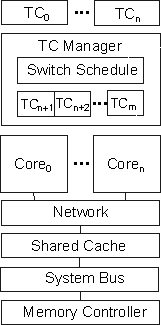
\includegraphics[width=1.08in]{figs/hw_sw_arch.pdf}
%        \caption{The Timing Compartments Architecture}
%        \label{fig:arch}
%    \end{center}
%\end{figure}

%As shown in Figure \ref{fig:arch}, the timing compartments architecture is 
%comprised of a set of $n$ cores which share resources. There is no limitation 
%on $m$, the number of timing compartments that can reside in the system at one 
%time. However, at most $n$ timing compartments can be active (executing on one 
%or more physical cores) at a time. If $m>n$, active timing compartments must 
%occasionally be switched with inactive ones. The TCM addresses this by context 
%switching TCs according to a context switch schedule.

\subsubsection{Hardware Control Interfaces}

%The hardware protection mechanisms in the previous section need to distinguish 
%memory accesses from different timing compartments.

%\subsubsection{TCIDs}

The hardware protection mechanisms track which timing compartment originated 
each request and handle the requests accordingly. Each core has a register that 
stores the timing compartment ID (TCID) of the TC currently active on that core. This is used to derive 
the tags that are appended to requests originating from that core. The TCID is 
$log\ n$ bits where $n$ is the number of cores in the processor.
Events such as network packets or cache accesses that use shared resources are 
tagged with the TCID of the corresponding core. 
The timing channel protection mechanisms use this TCID to distinguish accesses
from among different timing compartments.

For resource allocation, the hardware protection mechanisms allow the TCM to 
specify which timing compartment can use each partitioned resource.
For example, 
the partitioned cache includes $n$ registers that specify which cache partitions 
can be accessed for each timing compartment. 
%When a request requires a replacement, the cache uses the TCID of the request
%to decide which partitions can allow entries to be replaced according to the
%policy. (Checking is only required on replacements since TCIDs have separate
%address spaces.) 
In the set partitioned cache, the registers specify a mask
that is used to compute the cache array index from the memory address.
The mask maps accesses from each timing compartment to a subset of 
cache sets.
Similarly, each queue at the interface of the shared structures is tagged
with a TCID that owns that queue.
Table~\ref{table:tcid} summarizes the TCID registers in the system.

\begin{table}
\begin{center}
    \begin{footnotesize}
\begin{tabular}{l|l}
    \hline
    Component & TCID Storage \\
    \hline
    Core & $n$ cores. TCID register per core. \\
    \hline
    \multirow{3}{*}{Cache}
    & $n$ response queues. TCID register per queue \\
    & $n$ partition selection registers. \\
    & $n$ MSHR queues. TCID per queue\\
    \hline
    Network & $n$ queues. TCID register per queue\\
    \hline
    \multirow{2}{*}{Memory Controller}
    & $n$ request queues. TCID register per queue \\
    & $n$ response queues. TCID register per queue\\
    \hline
\end{tabular}
    \end{footnotesize}
    \caption{TCID registers for the shared structures.}
    \label{table:tcid}
\end{center}
\end{table}

For time-multiplexed resources, the hardware mechanisms contain control
registers so that the TCM can specify the schedule for time multiplexing.
More specifically, for an $n$-core system, a time-multiplexed resource
uses a schedule with $n$ time slices. Then, for each time slice, control
registers specify the length of the time slice in cycles, and
the TCID that is allowed to use the time slice. Finally, to support
coordination among related components, each time-multiplexed component
allows an offset to be specified by the TCM. The offset determines
the number of cycles before the first time slice starts after a reset.

%Each of the separate MSHR queues are tagged with a TCID of the owner, and 
%requests can only affect the MSHR queues with the same TCID as the request. 
%Each of the time multiplexed resources (the networks, the memory controller, 
%shared cache response ports, and memory controller response ports) have $n$ 
%queues.  Each of these queues has a register to store the TCID which owns that 
%particular queue. A time quantum is scheduled for each queue, so time quanta 
%are allocated to TCs by setting the queue configuration register with the TCID 
%of that TC. A single TC can be granted multiple queues, and therefore, multiple 
%time quanta in each rotation of the schedule. The configuration registers also 
%control the ordering of the queues in the schedule and the time offset of the 
%schedule. The offset delays the start of the schedule by some number of cycles 
%to allow the TDM schedules of multiple devices to be coordinated as described 
%in Section \ref{sec:coordination}. The configuration register can also set the 
%duration of the time quanta for each queue, but this cannot be changed based on 
%the dynamic behavior of the timing compartment.
%\subsubsection{Initialization \& Handling Context Switches}
%The TCM, initializes the system by setting the TCID storage elements listed in 
%Table 1 with the IDs of the initially active timing compartments. At most $n$ 
%of these can be active initially, so if $m>n$, some will be inactive, and the 
%TCM must define a static context switching schedule at initialization time.

\subsubsection{Context Switches}

% The time between context switches cannot depend on the dynamic behaviour of 
% the TCs. Otherwise, a timing compartment could observe the time that they are 
% context switched in or out to learn information about the timing compartment 
% it is switched with. Instead, context switches occur at a fixed time 
% interval, $T_{CTX}$. Every $T_{CTX}$ cycles the TCM is invoked to replace the 
% timing compartment which has been active the longest with the TC at the head 
% of the inactive TC queue. The compartment which has been switched out is 
% moved to the back of the inactive TC queue.

On a context switch, the TCM sets the TCID of a processing core to reflect
the incoming process (or virtual machine). The TCM also sets the control
registers for each protection mechanism to match the new set of active
timing compartments. Note that changing the resource allocation such as
partition sizes or time-multiplexing schedules may indicate
which process (or VM) is scheduled. However, it can be done independently
of secret data protected timing compartments (e.g. by allocating resources 
based on static performance characterizations).

For timing channel protection, the TCM also flushes per-core state elements
during a context switch.
Although private, per-core resources are not concurrently shared by TCs, they 
are shared across context switches. The state modified by the TC that is 
swapped out can affect the timing of the TC that is swapped in.
To perform the context switch, the CPU pipeline and the memory request queue 
are drained. 
%The general purpose registers of the outgoing TC are stored in 
%TCM-space memory and tagged with the TCID. 
The private cache, shared cache 
partition, TLB, and branch predictor state of the outgoing TC are all flushed.  
Finally, the TCID stores of the outgoing TC are replaced with the TCID of the 
incoming TC. 

%The time required to perform a context switch depends on the state and behavior 
%of the outgoing TC. The owner of the incoming TC can observe when the incoming 
%TC begins executing, so this implies a potential leakage of secrets. To 
%prevent this, context switches are bound to always take the worst case time.  
%If a context switch completes early, the incoming TC is stalled until the worst 
%case context switch time has been reached.

\subsection{Time Slice Coordination}
\label{sec:coordination}

The proposed architecture for implementing timing compartments rely heavily on
time division multiplexing of shared resources. For efficiency, the schedules
for adjacent time-multiplexed needs to be coordinated together to avoid 
unnecessary delays or wasted bandwidth.
%However, Naïvely time multiplexing the components with contention based timing channels 
%can lead to poor performance since many of these components are on the same 
%path to handle a request. 
% During a shared cache miss, the request is sent along the bus that connects 
% the private caches to the shared cache, which we refer to as the L2L3Bus.  
% After detecting the miss, a request is sent to memory through the bus 
% connecting the shared cache to the memory controller, which we refer to as 
% the membus. The memory controller handles the memory request and sends the 
% response back through the membus. Finally, the cache sends a response back 
% through the L2L3Bus.
%%%%%%% The NoC section should mention the request/response layers before this 
%%%%%%% section

%On the cache miss path both buses (which are each split into a request and 
%response layer), the response ports of the cache and memory controller, and the 
%memory controller itself are all time multiplexed. 

\begin{figure}
    \begin{center}
        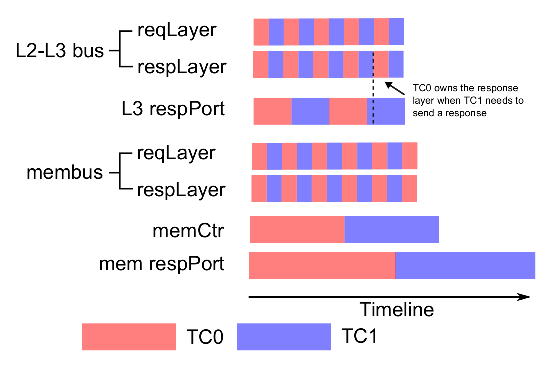
\includegraphics[width=3.46in]{figs/baseline_schedule.eps}
        \caption{Cache hit timing sequence.}
        \label{fig:naive_scheme}
    \end{center}
\end{figure}

Figure~\ref{fig:naive_scheme} illustrates a naïve time slice allocation that
does not consider interactions between related components.
In the figure, the L2-L3 bus is the bus connecting the private caches 
to the shared cache, and the membus connects the shared cache to the memory 
controller.
Unfortunately, the time slice allocation in the figure fails to properly
align time slices for common operations.
Notably, the L3 response port has its time slice misaligned with the L2-L3
bus. As a result, a response from L3 to L2 may have to unnecessarily delayed.
As a more subtle problem, the allocation uses the same time slices for both
request and response layers for the L2-L3 bus. However, an access to L3 has
a latency even in a cache hit. As a result, the response for a L3 request may
unnecessarily have to wait for the next time slice. 
%Ideally, the time slice
%for the response layer should be shifted to reflect the L3 access latency.

%Notably, the time quanta of each component are not aligned with each of the 
%L2-L3 bus time quanta.  During a shared cache hit on behalf of $TC1$, 
%occasionally the $TC1$ shared cache response port time quantum will be aligned 
%with the $TC1$ L2-L3 bus time quantum allowing it to proceed along the path 
%without unneeded stalls.  However, sometimes these are not well-aligned and 
%$TC1$ will have to wait for $TC2$ to finish before it can proceed. This becomes 
%even more wasteful
%as the number of timing compartments scales. A request may have to wait through 
%each other compartment's time quantum. 

\begin{figure}
    \begin{center}
        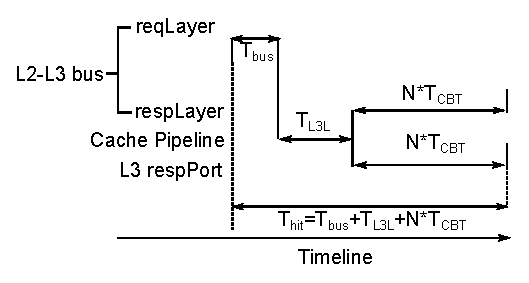
\includegraphics[width=2.4675in]{figs/hit_timing.eps}
        \caption{L3 cache hit timing sequence.}
        \label{fig:hit_timing}
    \end{center}
\end{figure}

To understand how the time slices for the L2-L3 interface need to be coordinated,
let us examine timing of a typical cache hit in Figure~\ref{fig:hit_timing},
which represents a common case. In this design, we assume that the cache is fully
pipelined and is capable of accepting a new request every cycle.
In the timing diagram, a request over the 
L2-L3 bus takes $T_{bus}$ cycles. The cache then takes $T_{L3L}$ cycles after 
receiving the request before the data is ready.
The response port transfers a cache block in $T_{CBT}$ cycles. 

\begin{figure}
    \begin{center}
        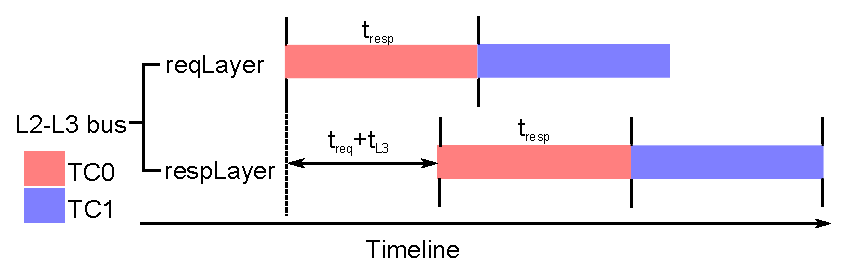
\includegraphics[width=3.2624in]{figs/hit_schedule.eps}
        \caption{Cache hit timing path schedule.}
        \label{fig:hit_schedule}
    \end{center}
\end{figure}

The goal of the time slice coordination is to maximize the chance of a 
request-response pair to proceed within a single time slice without the
response being blocked until the next turn.
Figure~\ref{fig:hit_schedule} shows the time slice allocation that matches 
the common cache hit timing. 
In the figure, the time slice for the response layer is shifted by $T_{bus} + T_{L3L}$
so that the response can use the L2-L3 bus after a cache access.
Also, the L3 response port uses the same time slice with the L2-L3 bus so that
both can be used at the same time.
To maintain that the relationship between the request and response layers,
the allocation uses the same time slice length for all three components.

%1) allow a request to proceed through common paths unblocked and 
%2) repeat this alignment for each TC. 
%Figure \ref{fig:hit_schedule} shows a 
%schedule that allows $N$ requests to proceed unblocked for each TCs turn. The 
%time quanta are aligned to follow the timings of \ref{fig:hit_timing}. To 
%guarantee that the behavior of a schedule repeats for the time quanta of each 
%TC, the durations of the time quanta for each resource must share a common 
%factor number of cycles. For example, if $N \times T_{CBT}$ (and this is the 
%time quanta duration for the response port and layer) is 16 and $T_{bus}$ is 3, 
%the actual time quanta duration for the request layer, $T_{req}$, should be 4, 
%8, or 16 even though the request port cannot do useful work for these extra 
%cycles. 

\begin{figure}
    \begin{center}
        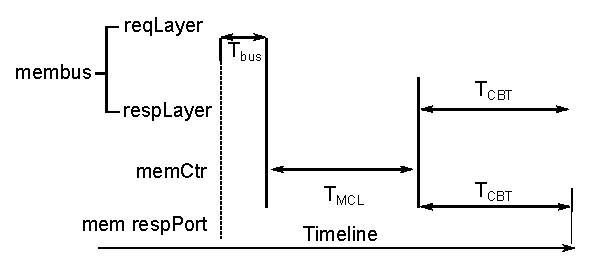
\includegraphics[width=2.9475in]{figs/miss_timing.eps}
        \caption{The L3-memory timing sequence.}
        \label{fig:miss_timing}
    \end{center}
\end{figure}

The analysis for the segment of the shared cache miss path between the shared 
cache and the memory controller is similar. The most significant difference is 
that unlike the cache, the memory controller itself is time multiplexed. Figure 
\ref{fig:miss_timing} shows the timing for this segment of the shared cache 
miss path. The time quanta of the memory controller have a duration that is 
chosen to be $T_{MCL}$. This optimal value may depend on the design, and
the authors of \cite{ushpca14} discuss the selection of this value. $M$ is the 
number of memory requests that can be handled in a single memory controller 
time quantum.
$T_{miss}$, the total period of the cache miss timing sequence is 
$T_{bus}+T_{MCL}+M\times T_{CBT}$.

The schedule of the entire system should allow the shared cache miss path to be 
traversed unblocked.
% , but since cache hits are more frequent than misses, the performance of the 
% cache hit path should not be weakened to meet this goal.
To prevent blocking along the request path, the time quantum of a timing 
compartment on the membus request port should begin just as that timing 
compartment's time quantum on the shared cache memory side request port 
finishes. This prevents blocking along the request path of the membus.
Similarly, to prevent blocking along the response path, the time quantum of the 
shared cache response port should begin just after the time quantum of the same 
timing compartment on the memory bus response layer ends. Figure 
\ref{fig:coordination}
shows a high level view of a full coordinated schedule.

\begin{figure}
    \begin{center}
        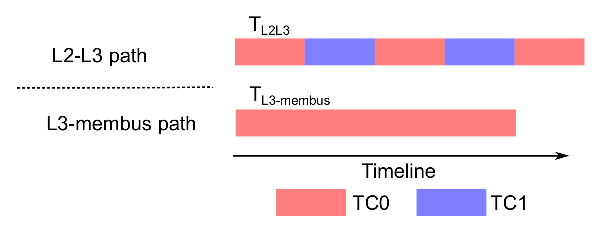
\includegraphics[width=2.9475in]{figs/coordination.eps}
        \caption{A coordinated cache miss path schedule.}
        \label{fig:coordination}
    \end{center}
\end{figure}

To meet the first criterion, the cache hit path timing sequence shown in 
\ref{fig:hit_timing} should be aligned with the start of the corresponding 
memory bus time quantum. To repeat this behavior for each cache hit path timing 
sequence, $T_{hit}$ and $T_{miss}$
should share a common factor. Since cache hits are more frequent than misses, 
the performance of the cache hit path should not be weakened to accomplish 
this. Instead, the length of the membus timing sequence should be increased 
(e.g. by increasing the memory controller time quantum). The second criterion 
is met if the maximum number of active timing compartments in the system (i.e.  
the number of cores) is a factor of the period of the membus timing sequence.
